\documentclass{article}

% Language setting
% Replace `english' with e.g. `spanish' to change the document language
\usepackage[english]{babel}
\usepackage{fontawesome5}
% Set page size and margins
% Replace `letterpaper' with `a4paper' for UK/EU standard size
\usepackage[letterpaper,top=2cm,bottom=2cm,left=3cm,right=3cm,marginparwidth=1.75cm]{geometry}

% Useful packages
\usepackage{amsmath}
\usepackage{graphicx}
\usepackage[colorlinks=true, allcolors=blue]{hyperref}

\title{Problem Set 6}
\author{JaeSeok Oh}

\begin{document}
	\maketitle
	
\begin{large}
\section*{Introduce Three Visualizations}

\begin{itemize}
	\item Introduction: This short report is about the data set I am interested in: the transactions of sneakers in StockX. Thanks to StockX Data Contest in Kaggle(url: \url{https://www.kaggle.com/datasets/hudsonstuck/stockx-data-contest}), I could easily download 99,956 observations from Jul 2017 to Feb 2019.
\end{itemize}

\begin{enumerate}
	\item First, I was wondering if the size of sneakers has an impact on sale prices - a seller might sell a pair at this price to a buyer, and vice versa. To think about this thought, one might be able to think that a pair of sneakers which is size 9-10 could be traded at the highest price due to the higher demand than the other sizes. Below is the plot and fitted values from the squared polynomial regression. The result seems reasonable, but it's difficult to conclude that shoe size alone has a significant impact.
	\begin{figure}[h]
		\centering
		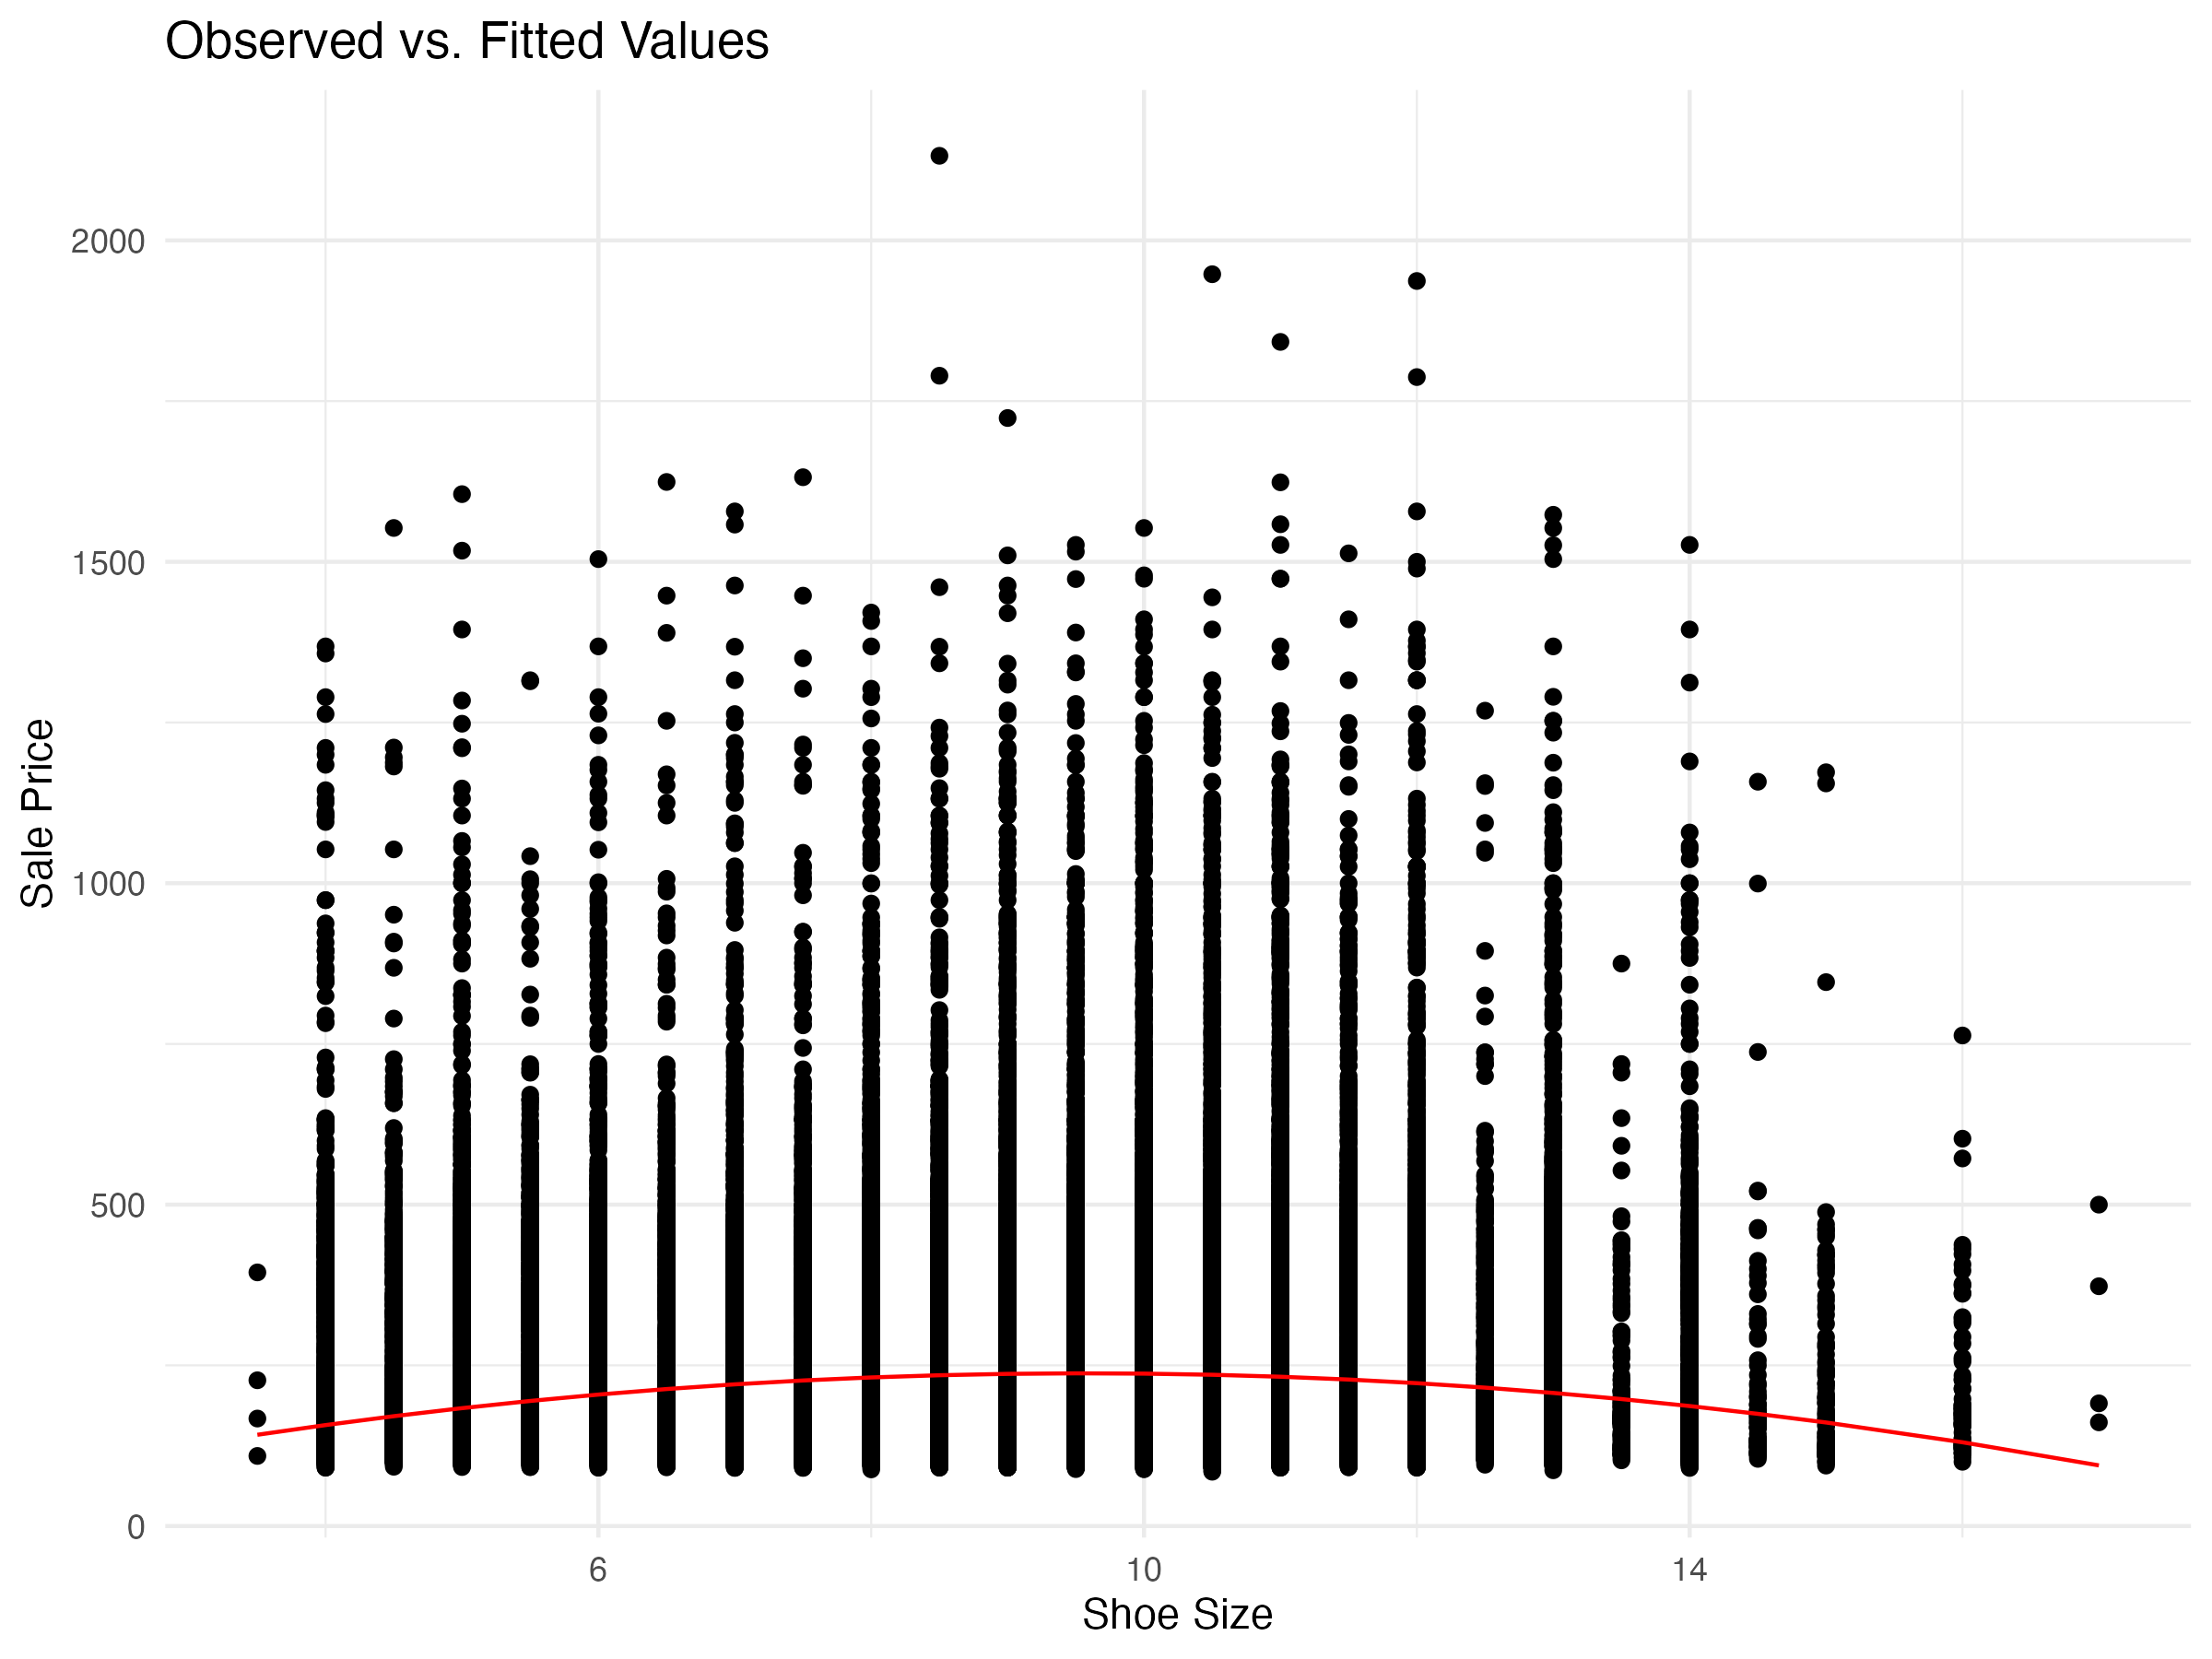
\includegraphics[width = 100mm]{PS6a_Oh.png}
	\end{figure}
	\item Second graph shows the price decreasing pattern over time. Note that I mark the order of transactions as a time dimension. For example, a pair of sneakers was traded 3 times in a day. I generate the `order' variable to set the order of transaction so that the pair has 1,2, and 3 times traded. This logic seems unreasonable since the other sizes and types of sneakers could not be marked in exactly the same time marking. However, it is sufficient because the beginning of this research requires to check the price pattern.
	\begin{figure}[h]
		\centering
		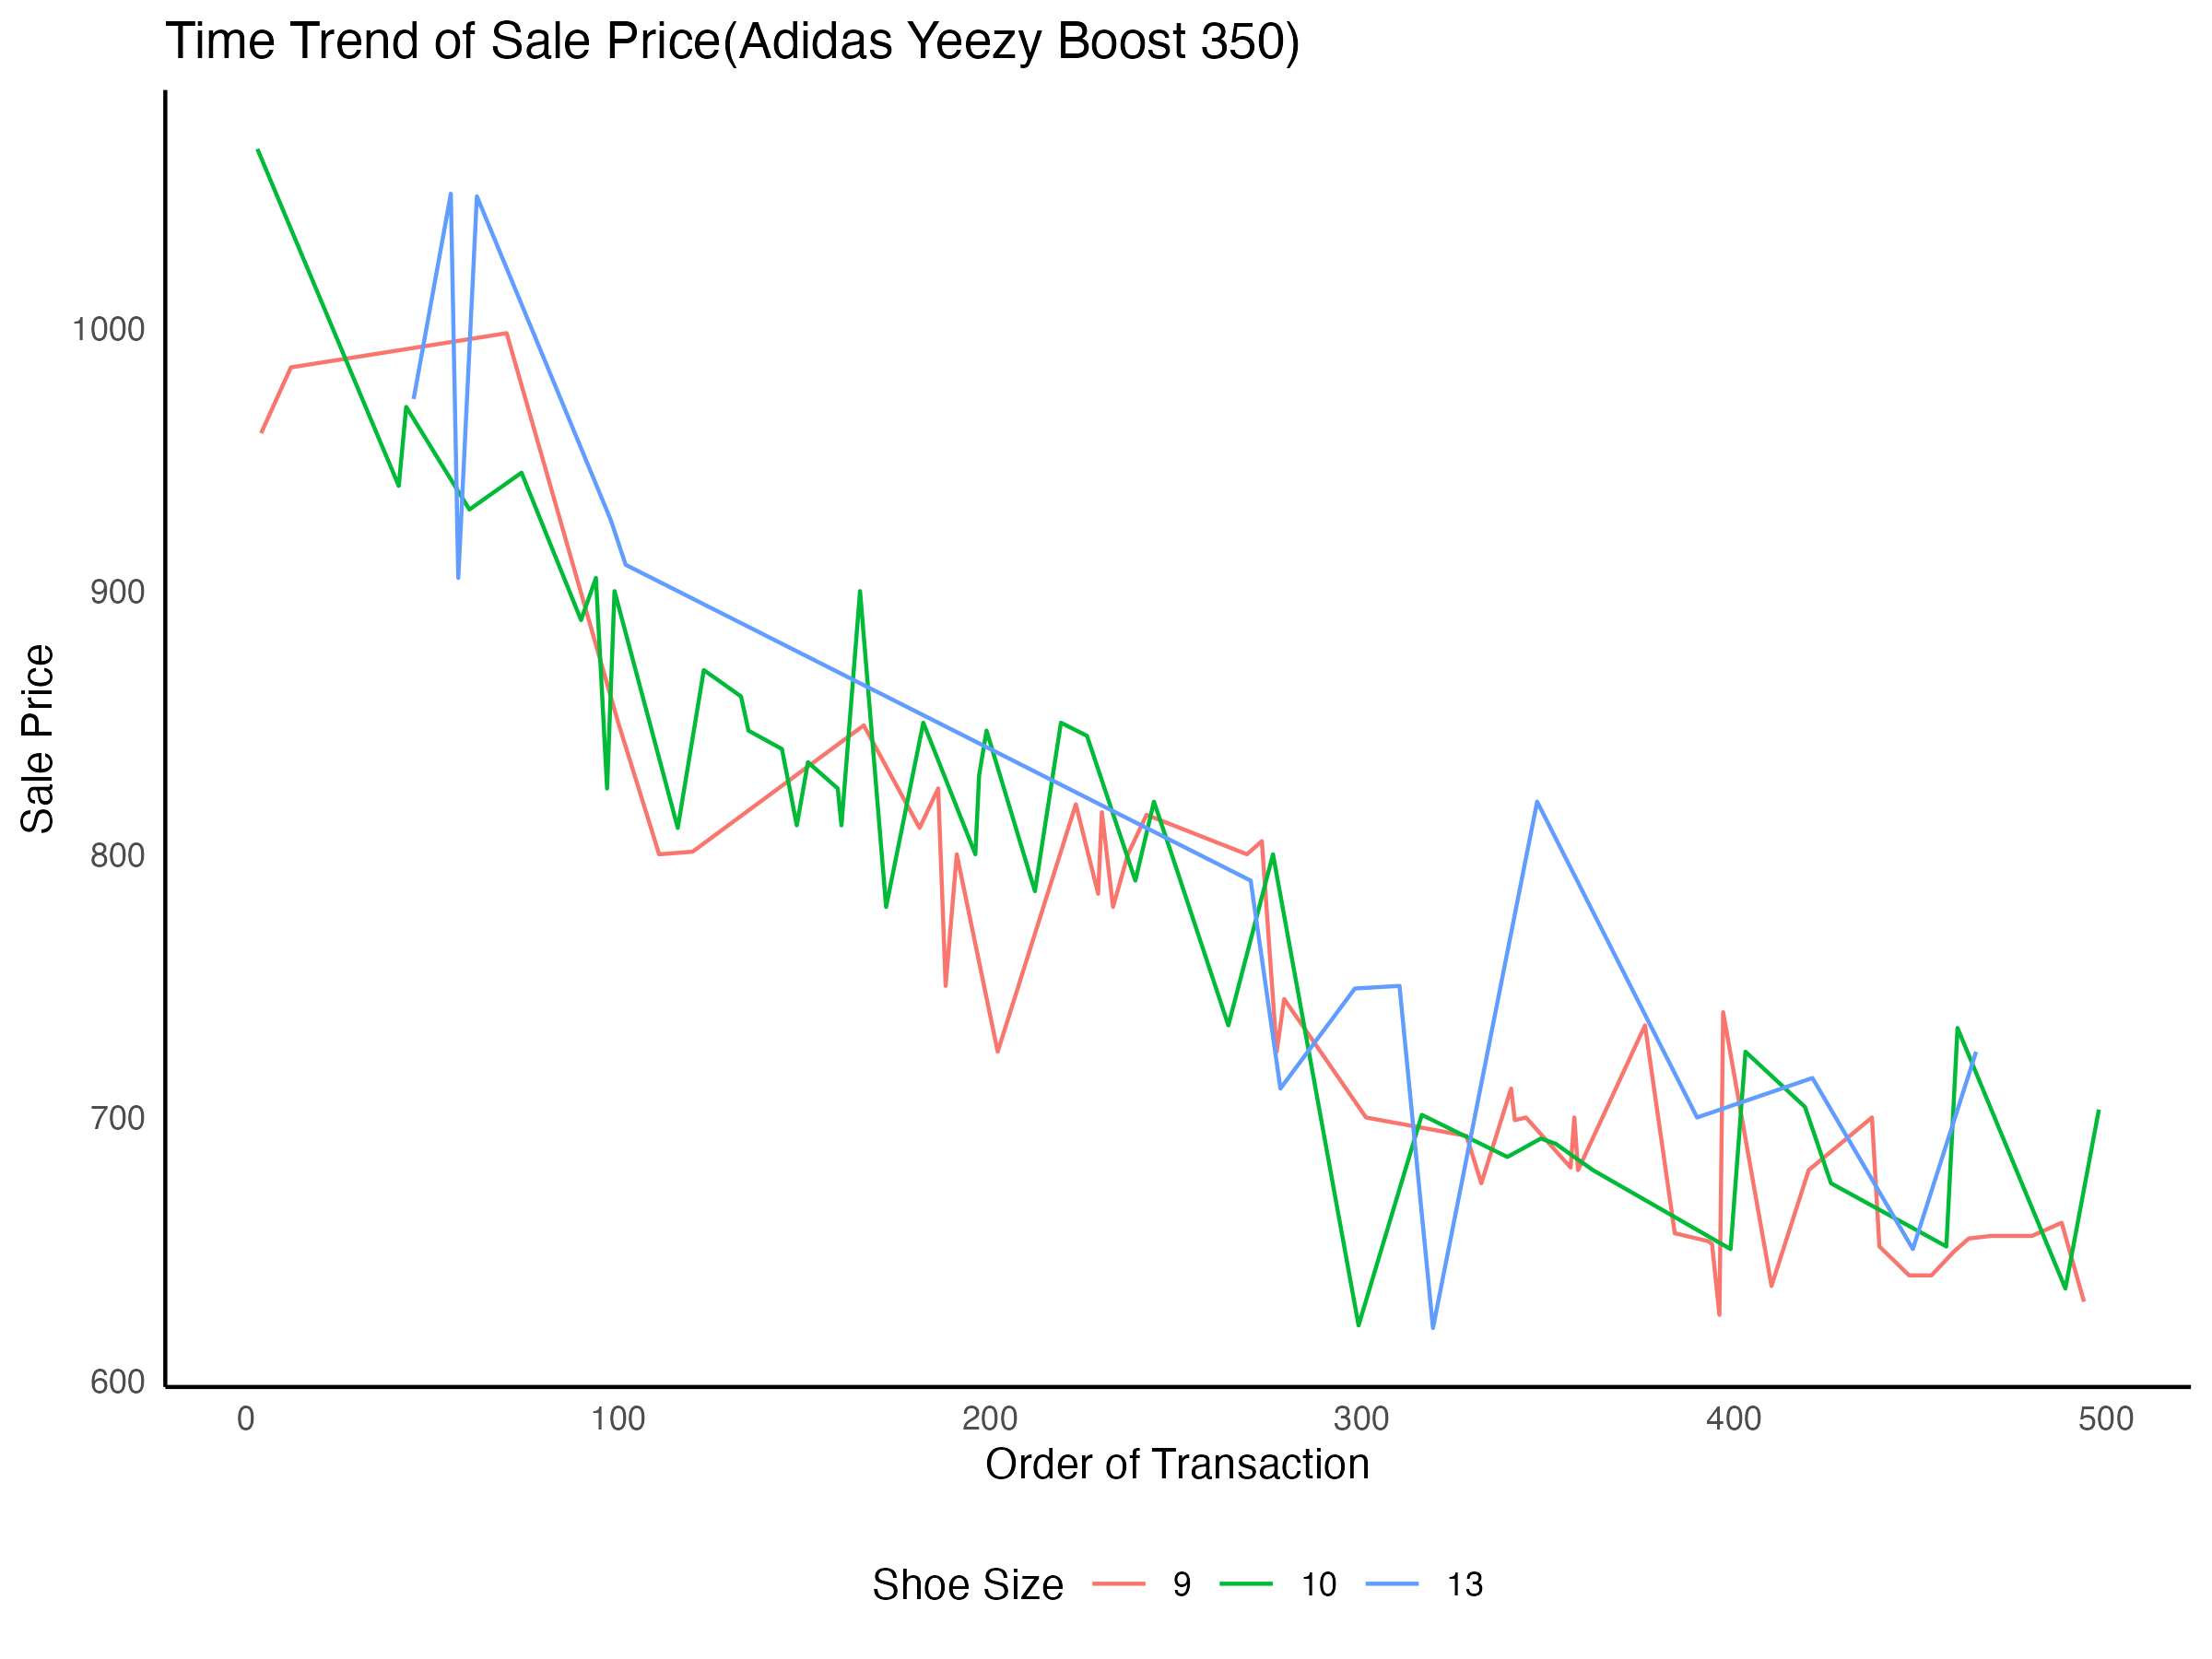
\includegraphics[width = 100mm]{PS6b_Oh.png}
	\end{figure}
	\item Finally, I draw a histogram to show which range of price is the most frequently sold. More than a half of transaction occurred less than \$1,000.
	\begin{figure}[h]
		\centering
		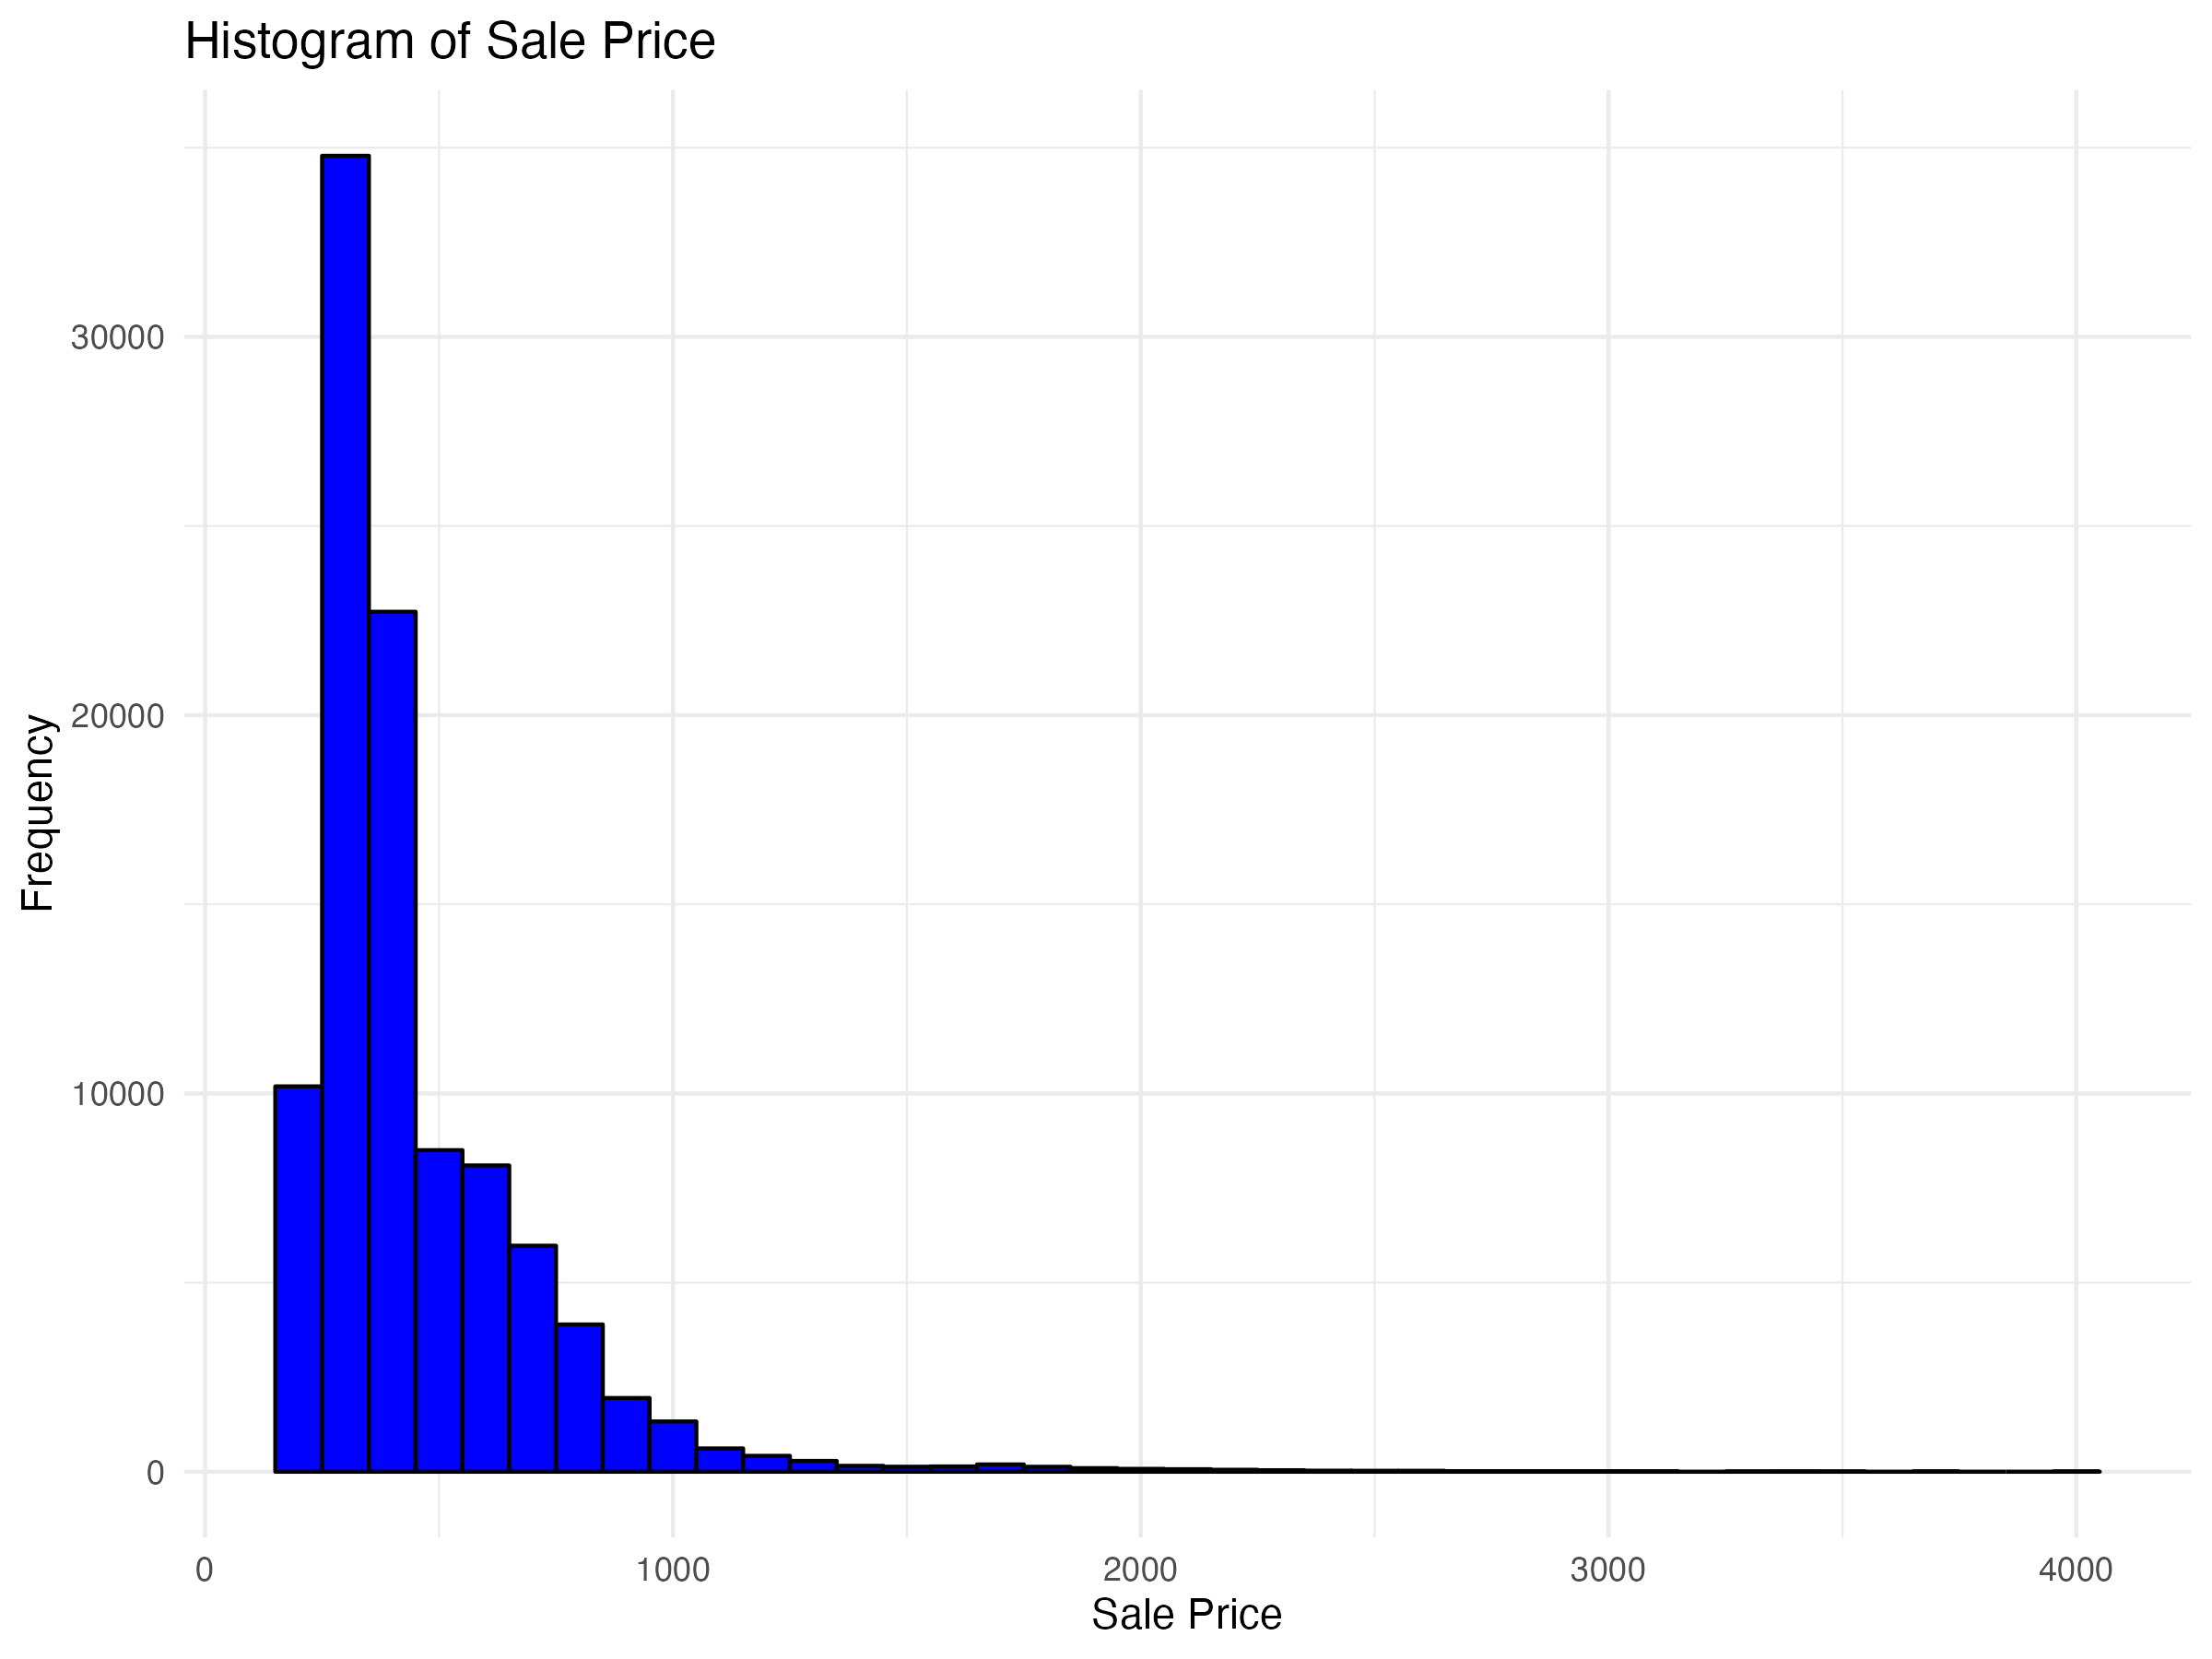
\includegraphics[width = 100mm]{PS6c_Oh.png}
	\end{figure}
\end{enumerate}




	
\end{large}
\end{document}